\documentclass[border=3pt,tikz]{standalone}
\usepackage[utf8]{vietnam}
\usetikzlibrary{calc,angles,intersections,shapes.geometric,arrows,decorations.markings,arrows.meta,patterns.meta,patterns}
\usepackage{tikz-3dplot,pgfplots}
\pgfplotsset{compat=1.15}
\usepgfplotslibrary{polar}
\usepackage{amsmath}
\begin{document}


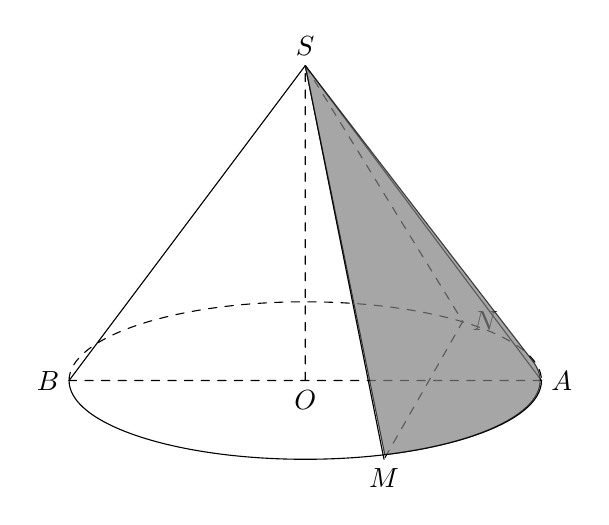
\begin{tikzpicture}[line
	join=round, line cap=round]
	\def\a{3}
	\def\b{1}
	\def\h{4}
	\draw[dashed] (180:\a) arc
	(180:0:{\a} and {\b});
	\draw (90:\h)--(180:\a)arc(180:360:{\a} and {\b})--cycle;
	\path
	(0,0) coordinate (O)
	(3,0) coordinate (A)
	(-3,0)coordinate (B)
	(2,0.75) coordinate (N) (1,-1) coordinate (M)
	(0,4) coordinate (S);
	\draw (S)--(M);
	\draw[dashed] (O)--(S)--(N)--(M) (A)--(B);
	\path (N) node[right] {$N$} (A) node[right] {$A$} (B) node[left] {$B$} (S) node[above] {$S$} (O) node[below] {$O$} (M) node[below] {$M$} ;
	\draw[fill=gray, opacity=0.7] (90:\h)--(317:0.46*\a)arc(290:375:{\a} and {\b})--cycle;
\end{tikzpicture}
\end{document}